\chapter{Introduction}
\section{Overview}

Obstacle k-Nearest Neighbour (OkNN) is a common type of spatial analysis query 
which can be described as follows: given a set of target points and a 
collection of polygonal obstacles, all in two dimensions, find the $k$ 
closest targets to an a priori unknown query point $q$.
Such problems appear in a myriad of practical contexts.
For example, in an industrial warehouse setting a machine operator may be
interested to know the $k$ closest storage locations where a specific 
inventory item can be found. In competitive computer games meanwhile, agent 
AIs often rely on nearest-neighbour information to make strategic decisions 
such as during navigation, combat or resource gathering.

\begin{figure}[htp]
  \centering
  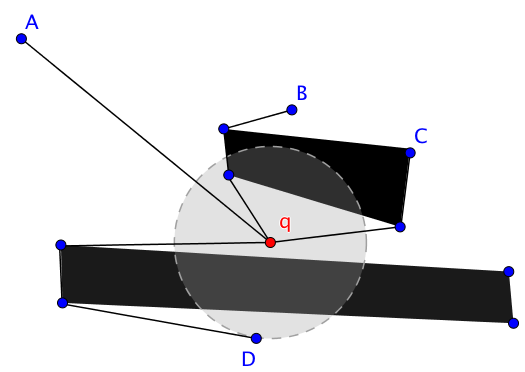
\includegraphics[width=\linewidth]{./pic/obs_dis.png}
  \caption{\small
  We aim to find the nearest neighbour of point $q$ from among the set of target points $A,B,C,D$. Black lines indicate the Euclidean shortest paths from $q$. Notice $D$ is the nearest neighbor of $q$ under the Euclidean metric but also the furthest neighbor of $q$ when obstacles are considered.}
\label{obs_dis}
\end{figure}

Traditional kNN queries in the plane (i.e. no obstacles) is a well studied
problem that can be handled by popular and well known algorithms including
~\textit{KD-Tree}~\cite{ooi1987spatial} and
\textit{R-tree}~\cite{guttman1984r}.  
%and other successful /variants\cite{beckmann1990r,sellis1987r+,kamel1993hilbert}).  
These methods organise the collection of target points into a hierarchical structure 
that serves to: (i) quickly identify a set of nearest neighbour candidates and; (ii) helps 
prune those candidates to return the $k$ closest.  A key ingredient to the success of
these algorithms is the Euclidean metric which provides perfect
distance information between any pair of points.  When obstacles are
introduced however the Euclidean metric becomes an often misleading
lower-bound. Figure~\ref{obs_dis} shows such an example.

Two popular algorithms for OkNN, which can deal with obstacles, are
\emph{local visibility graphs}~\cite{zhang2004spatial} and \emph{fast
filter}~\cite{xia2004fast}. Though different in details, both of these methods
are similar in that they depend on the incremental and online construction of 
a graph of co-visible points. Algorithms of this type are simple to understand, 
provide optimality guarantees and the promise of fast performance. 
Such advantages make incremental visibility graphs attractive to researchers 
and, despite more than a decade since their introduction, they continue to 
appear as ingredients in a variety of kNN studies from the literature; e.g. 
~\cite{gao2011efficient,gao2016reverse,gao2009continuous}.
However, incremental visibility graphs also suffer from a number of notable 
disadvantages including:
(i) online visibility checks;
(ii) an incremental construction process that has up to quadratic space and 
time complexity for the worst case;
(iii) duplicated effort, since the graph is discarded each time the query 
point changes.

In this paper we develop a new method for computing kNN in the presence of
obstacles which avoids these same disadvantages.  Our work extends
Polyanya~\cite{cuicompromise}: a recent and very fast algorithm for computing
Euclidean shortest paths on a navigation mesh: a data structure comprised of
convex polygons which taken together represent the entire traversable space.  
Compared to visibility graphs, navigation meshes are much cheaper to construct and
sometimes available as input ``for free'' (e.g. in computer game settings, navigation
meshes are often created, at least in part, by human designers).  
We describe how Polyanya can be generalised, from point-to-point problems to the
multi-target case. We also develop along the way two new, efficient and online heuristics
which can be used for OkNN.  Finally, we compare our work against incremental
visibility graphs in a wide range of experimental settings where we show that
Polyanya is in some cases three orders of magnitude faster.

The rest of the paper is organised as follows: (i) we give a description of the Obstacle kNN 
problem and associated technical terms; (ii) we review key components of
Polyanya; (iii) we give a formal description of our proposed algorithms including proofs and pseudocode;
(iv) experimental results and discussion and; (v) concluding thoughts.

